\section{Dataset details and Licenses}
\label{appendix:datadetails}
This section introduces the datasets and the motivation of downstream tasks.
\autoref{tab:dataset-stats} lists the licensing information and dataset size.


\begin{table}[h]
\resizebox{0.48\textwidth}{!}{%
\begin{tabular}{ll rrr}
\toprule
\textbf{Dataset} & \textbf{Licence} & \textbf{Train} & \textbf{Val\wpad} & \textbf{Test\wpad} \\
\midrule
\multicolumn{3}{l}{\textit{Phone Recognition}}\\
TIMIT & LDC & - & - & 6,300 \\
L2-ARCTIC & CC BY-NC 4.0 & - & - & 3,599 \\
Speech Accent Archive & CC BY-NC-SA 2.0 & - & - & 3,019 \\
DoReCo & CC0 1.0$^*$ & - & - & 18,734 \\
VoxAngeles & CC BY-NC 4.0 & - & - & 5,445 \\
Tusom2021 & MIT & - & - & 2,255 \\
\midrule
\multicolumn{3}{l}{\textit{Pathological Speech}}\\
{{EasyCall}} & CC BY-NC 2.0
 & 11,859 & 4,252 & 4,967 \\
{{UASpeech}} & \href{https://speechtechnology.web.illinois.edu/wp-content/uploads/2024/05/LICENSE.txt}{LICENSE}
 & 9,166 & 5,331 & 6,885 \\
{{UltraSuite}} & CC BY-NC 4.0
& 1,819 & 311 & 287 \\
\midrule
\multicolumn{3}{l}{\textit{L2 Speech}}\\
{{EdAcc}} & CC BY 4.0
& 6,917 & 2,525 & 5,497 \\
{{CMU Arctic}} & \href{http://www.festvox.org/cmu_arctic/cmu_arctic_report.pdf}{Free software}
& 2,264 & 1,132 & 1,132 \\
{{L2-ARCTIC}} & CC BY-NC 4.0
& 13,450 & 6,787 & 6,630 \\
{{SpeechOcean}} & CC BY 4.0
 & 2,260 & 240 & 2,500 \\
\midrule
\multicolumn{3}{l}{\textit{Multilingual Speech}}\\
{{FLEURS-24}} & CC BY 4.0
 & 4,800 & 2,400 & 4,800 \\
{{Vaani-Hi}} & CC-BY-4.0
 & 19,780 & 2,668 & 3,985 \\
 DoReCo & CC0 1.0$^*$ & - & - & 18,734 \\
\bottomrule
\end{tabular}
}
\caption{Licence and split size ($\#$utterance). $^*$DoReCo includes datasets of different CC licences; we use the 45-language subset created by \citet{zhu-etal-2024-taste}. See \autoref{appendix:datalinks} for dataset links.}
\label{tab:dataset-stats}
\end{table}

\subsection{Data Links}
\label{appendix:datalinks}
\begin{itemize}
    \item Phone Recognition datasets and EasyCall, EdAcc, CMU-Arctic, L2-ARCTIC, Fleurs-24 and Ultrasuite are available at \url{https://huggingface.co/collections/changelinglab/prism}
    \item UASpeech can be obtained from \url{https://speechtechnology.web.illinois.edu/uaspeech/}
    \item Speechocean762 can be downloaded from \url{https://github.com/jimbozhang/speechocean762}
\end{itemize}

\subsection{Datasets in Intrinsic Evaluation}
\label{appendix:datadetails-pr}
\paragraph{Variation in Seen Language}
TIMIT \citep{garofolo1993timit} contains speech from six regional varieties of American English and is often used for PR evaluation.
The Speech Accent Archive \citep{gmuspeechaccentarchive} provides read speech (the ``Please call Stella'' passage) and narrow phonetic transcriptions from non-native English speakers across 391 L1 languages.
L2-ARCTIC \cite{zhao2018l2arctic} includes read speech from non-native speakers; we use the L2-Arctic Perceived set\footnote{\url{https://huggingface.co/anyspeech}} which consists of manually annotated phoneme transcriptions rather than standard G2P output.

\paragraph{Unseen Languages}
DoReCo \citep{paschen2020doreco} is a dataset of 50+ small or endangered languages with broad phonetic transcriptions; we use the same DoReCo subset as \citet{zipa,zhu-etal-2024-taste}.
VoxAngeles \citep{chodroff2024voxangeles} is a cleaned, 95-language version of the UCLA Phonetics Lab Archive \citep{ucla2009}.
Tusom2021 \citep{mortensen2021tusom2021} is a dataset of speech and narrow phonetic transcriptions of individual words in the low-data Tangkhulic language Tusom. We removed tones as none of the models supports them.

\subsection{Datasets in Extrinsic Evaluation}
\label{appendix:datadetails-downstream}

\paragraph{Pathological Speech Assessment}
\textit{Dysarthria intelligibility prediction} predicts dysarthria severity levels based on phonetic representations. Increasing dysarthria severity is associated with reduced intelligibility, for which impaired phoneme production is a major clinical predictor \cite{xue2023assessing}. Two dysarthric speech datasets are evauated: UASpeech \cite{kim08c_interspeech}, an English corpus with speaker-level intelligibility scores, and EasyCall \cite{turrisi21_interspeech}, an Italian corpus annotated with dysarthria severity ratings. 
\textit{Child speech disorder detection} classifies whether a given utterance is produced by a child with speech disorder, supporting applications in speech therapy and the selection of specialized speech models \cite{rosero2025b, rosero2025a}.
We use acoustic recordings from the Ultrasuite corpus \cite{eshky2018ultrasuite}, with manually corrected transcription-audio mismatches. The curated dataset is released with this paper. %\drm{State how this is being evaluated.}

\paragraph{L2 Speech Evaluation}
\textit{Proficiency assessment for L2 Learners} uses phonetic information to automatically assess L2 English proficiency. We use utterances and sentence-level scores on a 0-10 scale from Speechocean762 \cite{zhang2021speechocean762opensourcenonnativeenglish}, an L1 Chinese, L2 English corpus. 
\textit{L1 influence classification} classifies a speaker’s L1 (native language) background, which introduces distinctive articulatory patterns into speech in an L2 language \cite{yang23_interspeech, shi21_icassp}.
We use EdAcc \cite{sanabria2023edacc} for one setup, and the other combines L2-ARCTIC \cite{zhao18_interspeech} for non-native speech with CMU ARCTIC \cite{kominek04_ssw} for native speech. %\drm{State how this is being evaluated.}

\paragraph{Multilingual Speech Identification}
\textit{Language identification} (LID) predicts the language spoken in an utterance from audio input. We use it as a coarse-grained evaluation of whether phonetic representations can distinguish both seen and unseen languages with the 102 languages in FLEURS \cite{conneau2023fleurs}.
\textit{Speech geolocation identification} predicts the origin of a speaker from an utterance in their native language, drawing on systematic phonetic shifts associated with geography, sociolinguistic variation, and language contact \citep{foley-2024-geolocating}. 
We use data from the Hindi-belt of India from Vaani \cite{vaani2025}. The detailed algorithm for this subset creation is explained in \autoref{appendix:vaani}.
\textit{Phone inventory induction} is the task of inferring the set of phones used by language from speech recordings, which is useful for language documentation and helps identify systematic errors during evaluation.
We use DoReCo (\autoref{appendix:phoneinv}) by deriving phone inventories from gold phone transcriptions and comparing them against the predicted transcriptions for each language.

\section{Metrics}
\subsection{Task Metric: F1 of Phone Inventory (F1-PI)}
\label{appendix:phoneinv}
A phone inventory is the set of all phones used in a language.
F1-PI assesses the degree of overlap between the phones transcribed by a system for a given language and the ground truth phone inventory for that language \citep{zelasko2022discovering}.
For two sets $A$ and $B$, the F1-score is defined as the harmonic mean of $|A-B|/|A|$ and $|B-A|/|B|$.
Set membership can be based on exact matches or fuzzy matches (e.g., over phonetic features).
This metric requires only a reference inventory for the target language, not a full transcription (although inventories can be derived from transcriptions), making it especially useful for under-resourced languages.

\subsection{Summary Metric: \bench Extrinsic Score}
\label{appendix:phonebenchscore}
To aggregate performance across extrinsic evaluation tasks with significantly varying test set sizes ($N_i$) (\autoref{tab:dataset-stats}), we compute a Score using a logarithmically weighted average. 
This approach ensures that larger datasets contribute more to the final score due to their statistical significance, while preventing them from completely dominating smaller, high-variance datasets (such as \texttt{CSD-us}).

Let $s_i$ be the model performance on task $i$ and $N_i$ be the number of samples in that task. The aggregate score $S$ is defined as:
\begin{equation}
    S = \frac{\sum_{i=1}^{K} \ln(N_i) \cdot s_i}{\sum_{i=1}^{K} \ln(N_i)}
\end{equation}
where $K=6$ corresponds to the tasks (\texttt{DYS-ez}, \texttt{DYS-ua}, \texttt{CSD-us}, \texttt{L1-eda}, \texttt{L1-arc}, and \texttt{L2-so}) that show differentiation in model behavior.
The weights $w_i = \ln(N_i)$ dampen the linear disparity between the largest ($N=7762$) and smallest ($N=287$) test sets.


\section{Experimental Setup}
\label{appendix:setup}

\paragraph{Probe Details}
All transcript probes use a 2 layer bi-directional GRU with mean pooling to get transcript level representation.
The GRU operates on a character vocabulary built from all predicted transcripts.
GRU has a hidden dimension of 256 and input dimension of 128 with a dropout of 0.1.

For hidden representation probes we use the last layer's hidden representation and attention pool over time to obtain utterance level representation.
This is followed by an MLP composed of 2 linear layers.
First layer's input dimension is the same as the dimension of the model being evaluated.
It outputs an embedding half of this size and the final layer outputs a single scalar for assessment taks, logits over classes for classification tasks, or a unit \texttt{[x y z]} vector for geolocation task.
MSE loss is employed for regression, cross-entropy for classification and angular error loss \cite{foley-2024-geolocating} for geolocation.

\paragraph{Hyper-parameters}
All the experiments can be reproduced via our open-sourced toollkit.
We use a learning rate of 2e-4 for all hidden representation probes and a learning rate of 1e-3 for the cascade probes.
We use the validation F1 (for classification), Kentall Tau (for assessment) and error (in km for geolocation) as early stopping metrics with a patience of 5 epochs and minimum epochs set to 10.
The checkpoint achieving best validation values on these metrics is selected for reporting numbers.

\paragraph{Compute spent}
Each TP probe runs in at most 15 minutes on a single 40GB GPU.
Each RP probe runs in at most 3 hours on a single 40GB GPU.
For TP and RP based extinsic evaluations a total of around 1k GPU hours were spent to get final numbers.
We used almost 1k GPU hours during development phase of the evaluation toolkit as well.
Besides, \bench supports distributed inference that scales to multiple GPUs and supports VLLM \footnote{\url{https://github.com/vllm-project/vllm}}.
For inference, we utilized around ~500 GPU hours including debugging and development costs.
Each \powsmctc model trains on 4 nodes with 4-80GB GPU each and takes 1.5 days to train, amounting to 600 GPU hours for one run.
We can assume another 2k GPU hours for development and experimentation.

\section{Prompts for LALMs}
\label{appendix:prompt}
{\small
\begin{promptbox}{PR: Phonetic Transcription (IPA)}
\textbf{System prompt}\par\vspace{2pt}
\noindent\#\#\# Role
\par
You are an expert phonetician and linguist specializing in acoustic phonetics. Your auditory perception is calibrated to detect subtle nuances in articulation, stress, and intonation.
\par\vspace{2pt}

\noindent\#\#\# Task
\par
Listen to the provided audio clip and transcribe the speech into standard International Phonetic Alphabet (IPA) symbols.
\par\vspace{2pt}

\noindent\#\#\# Guidelines for Accuracy
\par
\begin{itemize}[leftmargin=*,noitemsep,topsep=2pt]
  \item Analyze Context: Implicitly identify the speaker's accent/dialect to ensure vowel qualities are accurate.
  \item Resolve Ambiguity: If a sound is unclear, use your linguistic expertise to determine the single most probable phoneme. Do not provide alternatives.
  \item Strict IPA: Use standard IPA notation only.
\end{itemize}
\vspace{2pt}

\noindent\#\#\# Output Format \& Schema Adherence
\par
\begin{itemize}[leftmargin=*,noitemsep,topsep=2pt]
  \item Strict Adherence: You must generate the output following the defined schema structure exactly.
  \item Pure Data: Return raw data only. Do NOT use Markdown code blocks (e.g., \texttt{\string`\string`\string`json}), and do not include any conversational filler.
  \item Field \texttt{\string`\string`transcription\string`\string`}:
  \begin{itemize}[leftmargin=*,noitemsep,topsep=2pt]
    \item Must contain EXACTLY ONE string sequence of IPA symbols.
    \item No slashes \texttt{/} or brackets \texttt{[]}.
    \item Example: "\ipa{h@"l@U}" (Correct) / "/\ipa{h@"l@U}/" (Incorrect)
  \end{itemize}
\end{itemize}
\par\vspace{2pt}

Analyze the audio and produce the structured output now.

\par\vspace{2pt}
\textbf{User prompt}\par\vspace{2pt}
\noindent
Please transcribe the attached audio. I need a clear mapping of the speech to International Phonetic Alphabet (IPA) symbols.
\end{promptbox}

\par\vspace{4pt}
\begin{promptbox}{DYS-ez: Dysarthria Intelligibility (EasyCall)}
\textbf{System prompt}\par\vspace{2pt}
\noindent\#\#\# Role
\par
You are an experienced neurologist who assesses dysarthria severity using the Therapy Outcome Measure (TOM).
\par\vspace{2pt}

\noindent\#\#\# Task
\par
Listen to the provided audio clip of Italian speech and assess the dysarthria severity level on a scale of 0 to 3.
\par\vspace{2pt}

\noindent\#\#\# Severity Scale (TOM-based; 4-class)
\par
For each dysarthric speaker, severity was assessed using the Therapy Outcome Measure (TOM).
\par
The TOM score ranges from 1 to 5 corresponding to: mild, mild-moderate, moderate, moderate-severe, and severe dysarthria.
\par\vspace{2pt}

Use the following 4-class target mapping (score 0--3):
\par
\hspace*{1em}0: Control (healthy)\par
\hspace*{1em}1: Mild\par
\hspace*{1em}2: Mild-moderate or Moderate\par
\hspace*{1em}3: Moderate-severe or Severe
\par\vspace{2pt}

\noindent\#\#\# Output Format
\par
\begin{itemize}[leftmargin=*,noitemsep,topsep=2pt]
  \item Return JSON with a single field \texttt{\string`\string`score\string`\string`} containing an INTEGER from 0 to 3.
  \item Do NOT include any explanation, markdown, or extra text.
  \item If uncertain, give your best estimate within the valid range.
\end{itemize}

\par\vspace{2pt}
\textbf{User prompt}\par\vspace{2pt}
\noindent
Assess dysarthria severity using the TOM-based 4-class mapping: 0=Control (healthy), 1=Mild, 2=Mild-moderate or Moderate, 3=Moderate-severe or Severe. Output only the integer score (0-3).
\end{promptbox}

\par\vspace{4pt}
\begin{promptbox}{DYS-ua: Dysarthria Intelligibility (UASpeech)}
\textbf{System prompt}\par\vspace{2pt}
\noindent\#\#\# Role
\par
You assess speech intelligibility (severity of speech disorder) using a listener transcription accuracy based protocol.
\par\vspace{2pt}

\noindent\#\#\# Task
\par
Listen to the provided audio clip of English speech and predict the speaker's intelligibility category on a scale of 0 to 4.
\par\vspace{2pt}

\noindent\#\#\# Severity / Intelligibility Scale (5-class target)
\par
Speech intelligibility is used as an overall index of severity of dysarthria for each speaker and is based on word transcription tasks by human listeners.
\par
Based on averaged percent accuracy, each speaker is categorized into one of four intelligibility categories:
\par
\hspace*{1em}- very low (0--25\%)\par
\hspace*{1em}- low (26--50\%)\par
\hspace*{1em}- mid (51--75\%)\par
\hspace*{1em}- high (76--100\%)
\par\vspace{2pt}

Use the following 0--4 target encoding:
\par
\hspace*{1em}0: Control (healthy)\par
\hspace*{1em}1: High (76--100\%)\par
\hspace*{1em}2: Mid (51--75\%)\par
\hspace*{1em}3: Low (26--50\%)\par
\hspace*{1em}4: Very low (0--25\%)
\par\vspace{2pt}

\noindent\#\#\# Output Format
\par
\begin{itemize}[leftmargin=*,noitemsep,topsep=2pt]
  \item Return JSON with a single field \texttt{\string`\string`score\string`\string`} containing an INTEGER from 0 to 4.
  \item Do NOT include any explanation, markdown, or extra text.
  \item If uncertain, give your best estimate within the valid range.
\end{itemize}

\par\vspace{2pt}
\textbf{User prompt}\par\vspace{2pt}
\noindent
Predict the intelligibility category using the 0--4 mapping: 0=Control (healthy), 1=High (76--100\%), 2=Mid (51--75\%), 3=Low (26--50\%), 4=Very low (0--25\%). Output only the integer score (0-4).
\end{promptbox}

\par\vspace{4pt}
\begin{promptbox}{CSD-us: Child Speech Disorder (UltraSuite)}
\textbf{System prompt}\par\vspace{2pt}
\noindent\#\#\# Role
\par
You classify child speech from speech therapy session recordings as either typically developing speech or speech sound disorder speech.
\par\vspace{2pt}

\noindent\#\#\# Task
\par
Listen to the provided audio clip and classify the child speaker as either typically developing or having a speech sound disorder.
\par\vspace{2pt}

Notes:
\par
\hspace*{1em}- The child may hesitate, repeat, or make mistakes, and the spoken content may deviate from the prompt.
\par\vspace{2pt}

\noindent\#\#\# Class Mapping
\par
\hspace*{1em}0: Typical (typically developing child)\par
\hspace*{1em}1: Atypical (child with speech sound disorder)
\par\vspace{2pt}

\noindent\#\#\# Output Format
\par
\begin{itemize}[leftmargin=*,noitemsep,topsep=2pt]
  \item Return JSON with a single field \texttt{\string`\string`class\_id\string`\string`} containing either 0 (typical) or 1 (atypical).
  \item Do NOT include any explanation, markdown, or extra text.
\end{itemize}

\par\vspace{2pt}
\textbf{User prompt}\par\vspace{2pt}
\noindent
Classify the child speaker: 0=Typically developing, 1=Speech sound disorder. Output only the class\_id (0 or 1).
\end{promptbox}

\par\vspace{4pt}
\begin{promptbox}{L1-arc: L1 Classification (CMU-ARCTIC + L2-ARCTIC)}
\textbf{System prompt}\par\vspace{2pt}
\noindent\#\#\# Role
\par
You are an expert phonetician specializing in inferring a speaker's linguistic background from English speech. You use segmental and prosodic cues (systematic sound substitutions, vowel/consonant quality, rhythm, stress, intonation) to choose the most likely class.
\par\vspace{2pt}

\noindent\#\#\# Task
\par
Listen to the provided audio clip of non-native English speech and predict the speaker's native language (L1).
\par\vspace{2pt}

\noindent\#\#\# Class Mapping (class\_id \(\rightarrow\) native language)
\par
\hspace*{1em}0: Arabic (ar)\par
\hspace*{1em}1: English (en)\par
\hspace*{1em}2: Spanish (es)\par
\hspace*{1em}3: Hindi (hi)\par
\hspace*{1em}4: Korean (ko)\par
\hspace*{1em}5: Vietnamese (vi)\par
\hspace*{1em}6: Chinese/Mandarin (zh)
\par\vspace{2pt}

\noindent\#\#\# Guidelines
\par
\begin{itemize}[leftmargin=*,noitemsep,topsep=2pt]
  \item Focus on segmental cues (vowels/consonants) and systematic substitutions.
  \item Focus on prosodic cues (rhythm, stress, intonation).
  \item Use ONLY the class mapping above; output EXACTLY ONE class\_id.
  \item If uncertain, output your single best class\_id (no hedging).
\end{itemize}

\noindent\#\#\# Output Format
\par
\begin{itemize}[leftmargin=*,noitemsep,topsep=2pt]
  \item Return JSON with a single field \texttt{\string`\string`class\_id\string`\string`} containing an integer from 0 to 6.
  \item Do NOT include any explanation, markdown, or extra text.
\end{itemize}

\par\vspace{2pt}
\textbf{User prompt}\par\vspace{2pt}
\noindent
Listen to this English speech and predict the speaker's native language. Output only the class\_id.
\end{promptbox}

\par\vspace{4pt}
\begin{promptbox}{L1-eda: L1 Classification (EdAcc)}
\textbf{System prompt}\par\vspace{2pt}
\noindent\#\#\# Role
\par
You are an expert phonetician specializing in inferring a speaker's linguistic background from English speech. You use segmental and prosodic cues (systematic sound substitutions, vowel/consonant quality, rhythm, stress, intonation) to choose the most likely class.
\par\vspace{2pt}

\noindent\#\#\# Task
\par
Listen to the provided audio clip of English speech and classify the speaker's accent into one of 13 accent clusters.
\par\vspace{2pt}

\noindent\#\#\# Class Mapping (class\_id \(\rightarrow\) accent cluster)
\par
Output EXACTLY ONE class\_id from the fixed mapping below.
\par\vspace{2pt}

\hspace*{1em}0: AFRICAN\_ENGLISH\par
\hspace*{1em}1: AFROASIATIC\_SEMITIC\par
\hspace*{1em}2: CARIBBEAN\par
\hspace*{1em}3: CELTIC\_ENGLISH\par
\hspace*{1em}4: EAST\_ASIAN\par
\hspace*{1em}5: GALLO\_ROMANCE\par
\hspace*{1em}6: GERMANIC\par
\hspace*{1em}7: INNER\_CIRCLE\_ENGLISH\par
\hspace*{1em}8: INSULAR\_SEA\par
\hspace*{1em}9: MAINLAND\_SEA\par
\hspace*{1em}10: ROMANCE\par
\hspace*{1em}11: SLAVIC\_BALKAN\par
\hspace*{1em}12: SOUTH\_ASIAN
\par\vspace{2pt}

\noindent\#\#\# Guidelines
\par
\begin{itemize}[leftmargin=*,noitemsep,topsep=2pt]
  \item Focus on segmental cues (vowels/consonants) and systematic substitutions.
  \item Focus on prosodic cues (rhythm, stress, intonation).
  \item Use ONLY the class mapping above; output EXACTLY ONE class\_id.
  \item If uncertain, output your single best class\_id (no hedging).
\end{itemize}

\noindent\#\#\# Output Format
\par
\begin{itemize}[leftmargin=*,noitemsep,topsep=2pt]
  \item Return JSON with a single field \texttt{\string`\string`class\_id\string`\string`} containing an integer from 0 to 12.
  \item Do NOT include any explanation, markdown, or extra text.
\end{itemize}

\par\vspace{2pt}
\textbf{User prompt}\par\vspace{2pt}
\noindent
Listen to this English speech and classify the speaker's accent cluster. Output only the class\_id (0-12).
\end{promptbox}

\par\vspace{4pt}
\begin{promptbox}{L2-so: L2 Proficiency (Speechocean762)}
\textbf{System prompt}\par\vspace{2pt}
\noindent\#\#\# Role
\par
You are an expert rater of non-native English speech. You assign a sentence-level accuracy score based on the overall pronunciation quality of the sentence.
\par\vspace{2pt}

\noindent\#\#\# Task
\par
Listen to the provided audio clip and rate the sentence-level accuracy on an integer scale from 0 to 10.
\par\vspace{2pt}

\noindent\#\#\# Sentence-level Accuracy Scoring (0--10)
\par
\hspace*{1em}9-10: The overall pronunciation of the sentence is excellent without obvious mispronunciation\par
\hspace*{1em}7-8: The overall pronunciation of the sentence is good, with a few mispronunciations\par
\hspace*{1em}5-6: The pronunciation of the sentence has many mispronunciations but it is still understandable\par
\hspace*{1em}3-4: Awkward pronunciation with many serious mispronunciations\par
\hspace*{1em}0-2: The pronunciation of the whole sentence is unable to understand or there is no voice
\par\vspace{2pt}

\noindent\#\#\# Output Format
\par
\begin{itemize}[leftmargin=*,noitemsep,topsep=2pt]
  \item Return JSON with a single field \texttt{\string`\string`score\string`\string`} containing an INTEGER from 0 to 10.
  \item Do NOT include any explanation, markdown, or extra text.
  \item If uncertain, give your best estimate within the valid range.
\end{itemize}

\par\vspace{2pt}
\textbf{User prompt}\par\vspace{2pt}
\noindent
Rate the sentence-level pronunciation accuracy on an integer scale of 0-10. Output only the integer score.
\end{promptbox}

\par\vspace{4pt}
\begin{promptbox}{LID-fl: LID (FLEURS)}
\textbf{System prompt}\par\vspace{2pt}
\noindent\#\#\# Role
\par
You are an expert phonetician specializing in inferring linguistic background from speech. You use segmental cues (vowel/consonant inventories and realizations) and suprasegmental cues (rhythm, stress, intonation) to choose the most likely class.
\par\vspace{2pt}

\noindent\#\#\# Task
\par
Listen to the provided audio clip and identify which of the 24 languages is being spoken.
\par\vspace{2pt}

\noindent\#\#\# Class Mapping (class\_id \(\rightarrow\) language)
\par
Output EXACTLY ONE class\_id from the fixed mapping below.
\par\vspace{2pt}

\hspace*{1em}0: Assamese\par
\hspace*{1em}1: Asturian\par
\hspace*{1em}2: Persian\par
\hspace*{1em}3: Filipino\par
\hspace*{1em}4: Gujarati\par
\hspace*{1em}5: Hebrew\par
\hspace*{1em}6: Armenian\par
\hspace*{1em}7: Igbo\par
\hspace*{1em}8: Kamba\par
\hspace*{1em}9: Kabuverdianu\par
\hspace*{1em}10: Khmer\par
\hspace*{1em}11: Kannada\par
\hspace*{1em}12: Sorani-Kurdish\par
\hspace*{1em}13: Luxembourgish\par
\hspace*{1em}14: Ganda\par
\hspace*{1em}15: Lingala\par
\hspace*{1em}16: Luo\par
\hspace*{1em}17: Latvian\par
\hspace*{1em}18: Nepali\par
\hspace*{1em}19: Northern-Sotho\par
\hspace*{1em}20: Occitan\par
\hspace*{1em}21: Pashto\par
\hspace*{1em}22: Umbundu\par
\hspace*{1em}23: Wolof
\par\vspace{2pt}

\noindent\#\#\# Guidelines
\par
\begin{itemize}[leftmargin=*,noitemsep,topsep=2pt]
  \item Focus on segmental cues (vowels/consonants) and systematic realizations.
  \item Focus on suprasegmental cues (rhythm, stress, intonation) and phonotactics.
  \item Use ONLY the class mapping above; output EXACTLY ONE class\_id.
  \item If uncertain, output your single best class\_id (no hedging).
\end{itemize}

\noindent\#\#\# Output Format
\par
\begin{itemize}[leftmargin=*,noitemsep,topsep=2pt]
  \item Return JSON with a single field \texttt{\string`\string`class\_id\string`\string`} containing an integer from 0 to 23.
  \item Do NOT include any explanation, markdown, or extra text.
\end{itemize}

\par\vspace{2pt}
\textbf{User prompt}\par\vspace{2pt}
\noindent
Identify the language. Use ONLY the class mapping above and output exactly one class\_id (0-23).
\end{promptbox}

\par\vspace{4pt}
\begin{promptbox}{GEO-v: Speech Geolocation (Vaani)}
\textbf{System prompt}\par\vspace{2pt}
\noindent\#\#\# Role
\par
You are an expert dialectologist. You infer a speaker's geographic origin from dialectal cues in speech.
\par\vspace{2pt}

\noindent\#\#\# Task
\par
Listen to the provided audio clip and predict the speaker's geographic location from dialectal features.
\par\vspace{2pt}

\noindent\#\#\# Output
\par
Return JSON only with latitude/longitude in decimal degrees:
\par
\hspace*{1em}- \texttt{\{ "lat": NUMBER, "lon": NUMBER \}}\par
\hspace*{1em}- lat in \texttt{[-90, 90]}, lon in \texttt{[-180, 180]}\par
\hspace*{1em}- Do NOT include any explanation or extra text.
\par\vspace{2pt}

\textbf{User prompt}\par\vspace{2pt}
\noindent
Predict the geographic location. Output JSON only: \texttt{\{ "lat": <deg>, "lon": <deg> \}}.
\end{promptbox}

\ifdefined\linenumbers\linenumbers\fi
}



\section{L1 to accent cluster mapping for EdAcc}
The EdAcc corpus contains 41 distinct L1 labels, which we consolidate into 13 accent clusters based on phonological and typological similarity.
Grouping criteria include language family (e.g., Sino-Tibetan, Austronesian), vowel inventory size (e.g., 5-vowel Romance languages), prosodic patterns (e.g., syllable-timed vs.\ stress-timed), and shared phonetic transfer patterns to English (e.g., rhoticity, vowel reduction).
\autoref{tab:edacc-l1-accent-mapping} lists the complete mapping.

\label{appendix:edacc-l1-accent-mapping}
\begin{table}[t]
\centering
\scriptsize
\setlength{\tabcolsep}{6pt}
\begin{tabular}{l l}
\toprule
\textbf{EdAcc L1 label} & \textbf{Accent cluster} \\
\midrule
Hindi & SOUTH\_ASIAN \\
Indian English & SOUTH\_ASIAN \\
Urdu & SOUTH\_ASIAN \\
Sinhalese & SOUTH\_ASIAN \\
\midrule
English & INNER\_CIRCLE\_ENGLISH \\
Southern British English & INNER\_CIRCLE\_ENGLISH \\
Mainstream US English & INNER\_CIRCLE\_ENGLISH \\
South African English & INNER\_CIRCLE\_ENGLISH \\
\midrule
Scottish English & CELTIC\_ENGLISH \\
Irish English & CELTIC\_ENGLISH \\
\midrule
Spanish & ROMANCE \\
Spanish (Mexican) & ROMANCE \\
Catalan & ROMANCE \\
Italian & ROMANCE \\
Portoguese & ROMANCE \\
Maltese & ROMANCE \\
\midrule
French & GALLO\_ROMANCE \\
\midrule
Indonesian & INSULAR\_SEA \\
Bahasa & INSULAR\_SEA \\
Filipino & INSULAR\_SEA \\
Tagalog & INSULAR\_SEA \\
\midrule
Vietnamese & MAINLAND\_SEA \\
\midrule
Mandarin & EAST\_ASIAN \\
Japanese & EAST\_ASIAN \\
Korean & EAST\_ASIAN \\
\midrule
Nigerian English & AFRICAN\_ENGLISH \\
Kenyan English & AFRICAN\_ENGLISH \\
Ghanain English & AFRICAN\_ENGLISH \\
\midrule
Russian & SLAVIC\_BALKAN \\
Polish & SLAVIC\_BALKAN \\
Bulgarian & SLAVIC\_BALKAN \\
Macedonian & SLAVIC\_BALKAN \\
Montenegrin & SLAVIC\_BALKAN \\
Lithuanian & SLAVIC\_BALKAN \\
Romanian & SLAVIC\_BALKAN \\
\midrule
German & GERMANIC \\
Dutch & GERMANIC \\
Icelandic & GERMANIC \\
\midrule
Arabic & AFROASIATIC\_SEMITIC \\
Hebrew & AFROASIATIC\_SEMITIC \\
\midrule
Jamaican English & CARIBBEAN \\
\bottomrule
\end{tabular}
\caption{Mapping from EdAcc L1 labels (41) to 13 accent clusters used in \texttt{L1-eda}.}
\label{tab:edacc-l1-accent-mapping}
\end{table}

\section{Algorithm for Vaani-Hi}
\label{appendix:vaani}

For the \texttt{GEO-v} task, we construct \textbf{Vaani-Hi}, a Hindi-belt subset of the Vaani corpus \citep{vaani2025}, and release it on Hugging Face.

\paragraph{Sampling}
We focus on 12 Hindi-belt states: Chandigarh, Himachal Pradesh, Delhi, Madhya Pradesh, Jharkhand, Uttarakhand, Bihar, Chhattisgarh, Haryana, Rajasthan, Punjab, and Uttar Pradesh.
From each state, we randomly sample up to 4 districts; for each district, we use up to 4 audio shards and take up to 600 utterances per shard (seed 42).

\paragraph{Filtering and Labeling}
We retain only pincodes with more than 450 utterances to ensure sufficient density per location.
Each pincode is mapped to latitude/longitude using a pincode metadata table; we assign mean coordinates per pincode as the geolocation target.

\paragraph{Splitting and Preprocessing}
Splits are created within each pincode (75\%/10\%/15\% train/val/test) to avoid location leakage.
Audio is resampled to 16\,kHz and clipped to a maximum of 20 seconds.


\section{Effect of Thinking Mode on L1-eda Classification}
\label{appendix:lalm-confusion}

\autoref{fig:lalm-cm} provides the full confusion matrices for the LALM bias analysis discussed in \S\ref{sec:mallm}.

\begin{figure}[h]
  \centering
  \begin{subfigure}[b]{0.48\textwidth}
    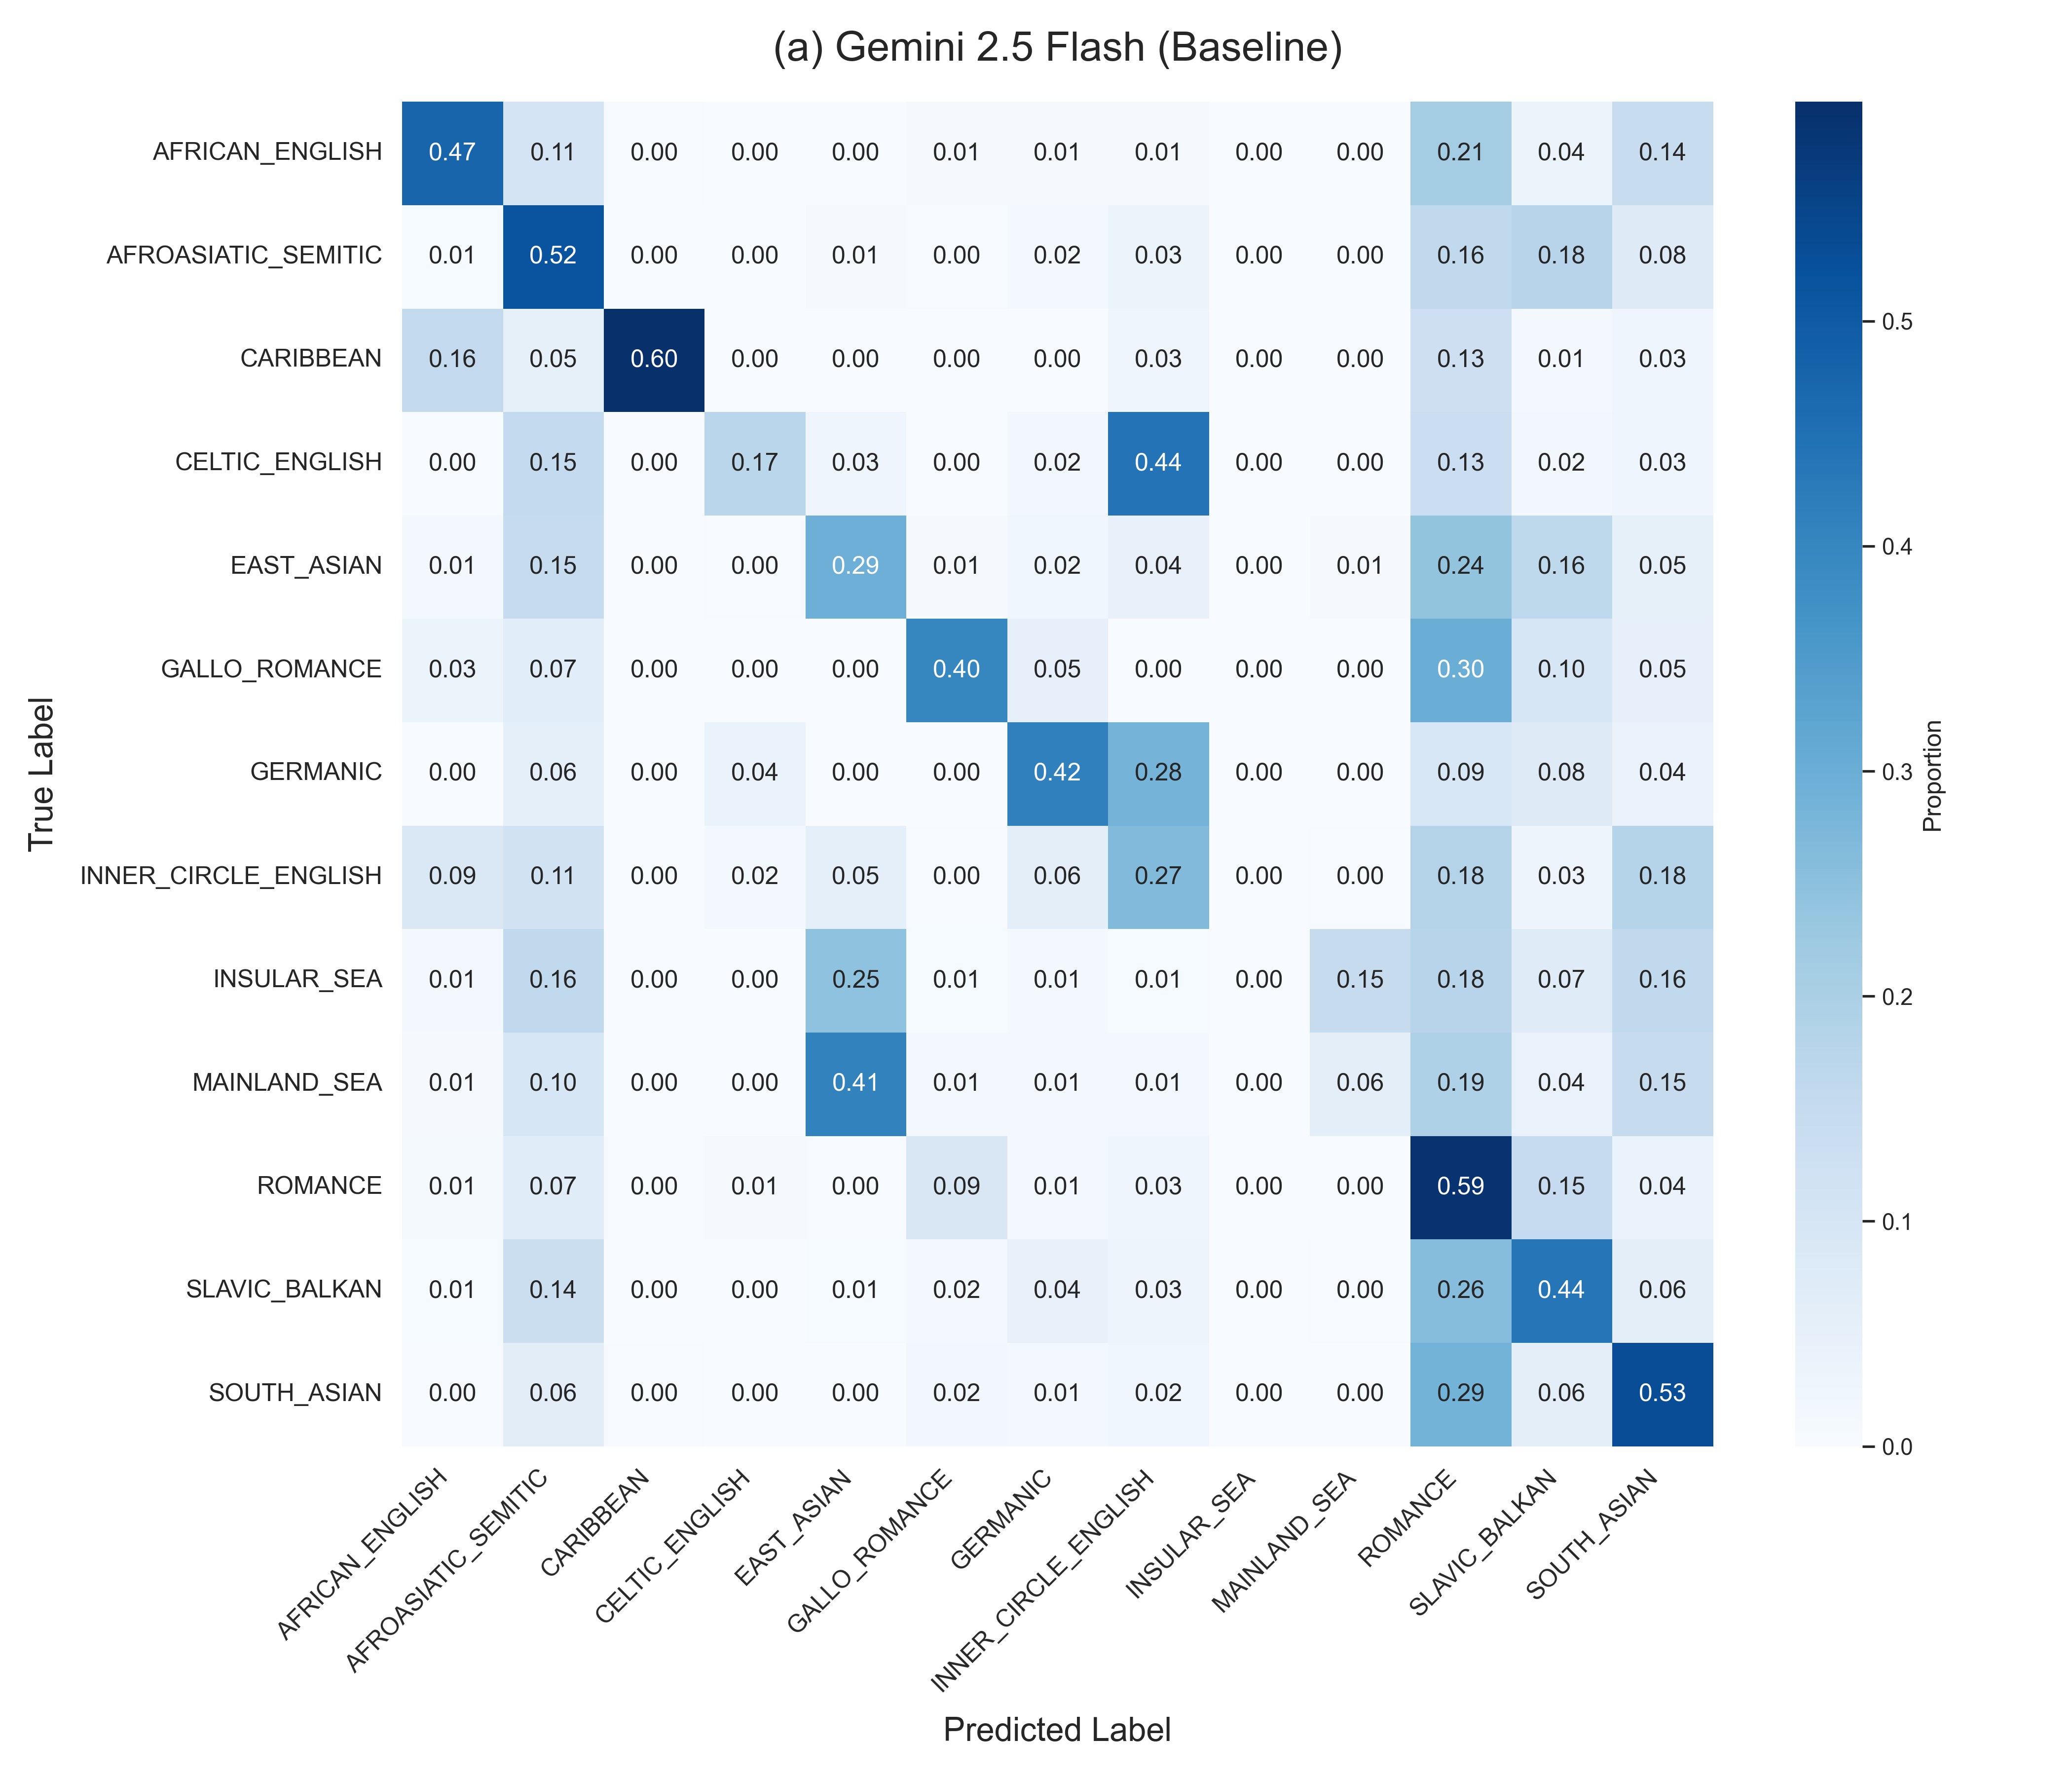
\includegraphics[width=\textwidth]{figures/cm_gemini_baseline.png}
    \caption{Baseline (F1-score=32.7\%)}
  \end{subfigure}
  \hfill
  \begin{subfigure}[b]{0.48\textwidth}
    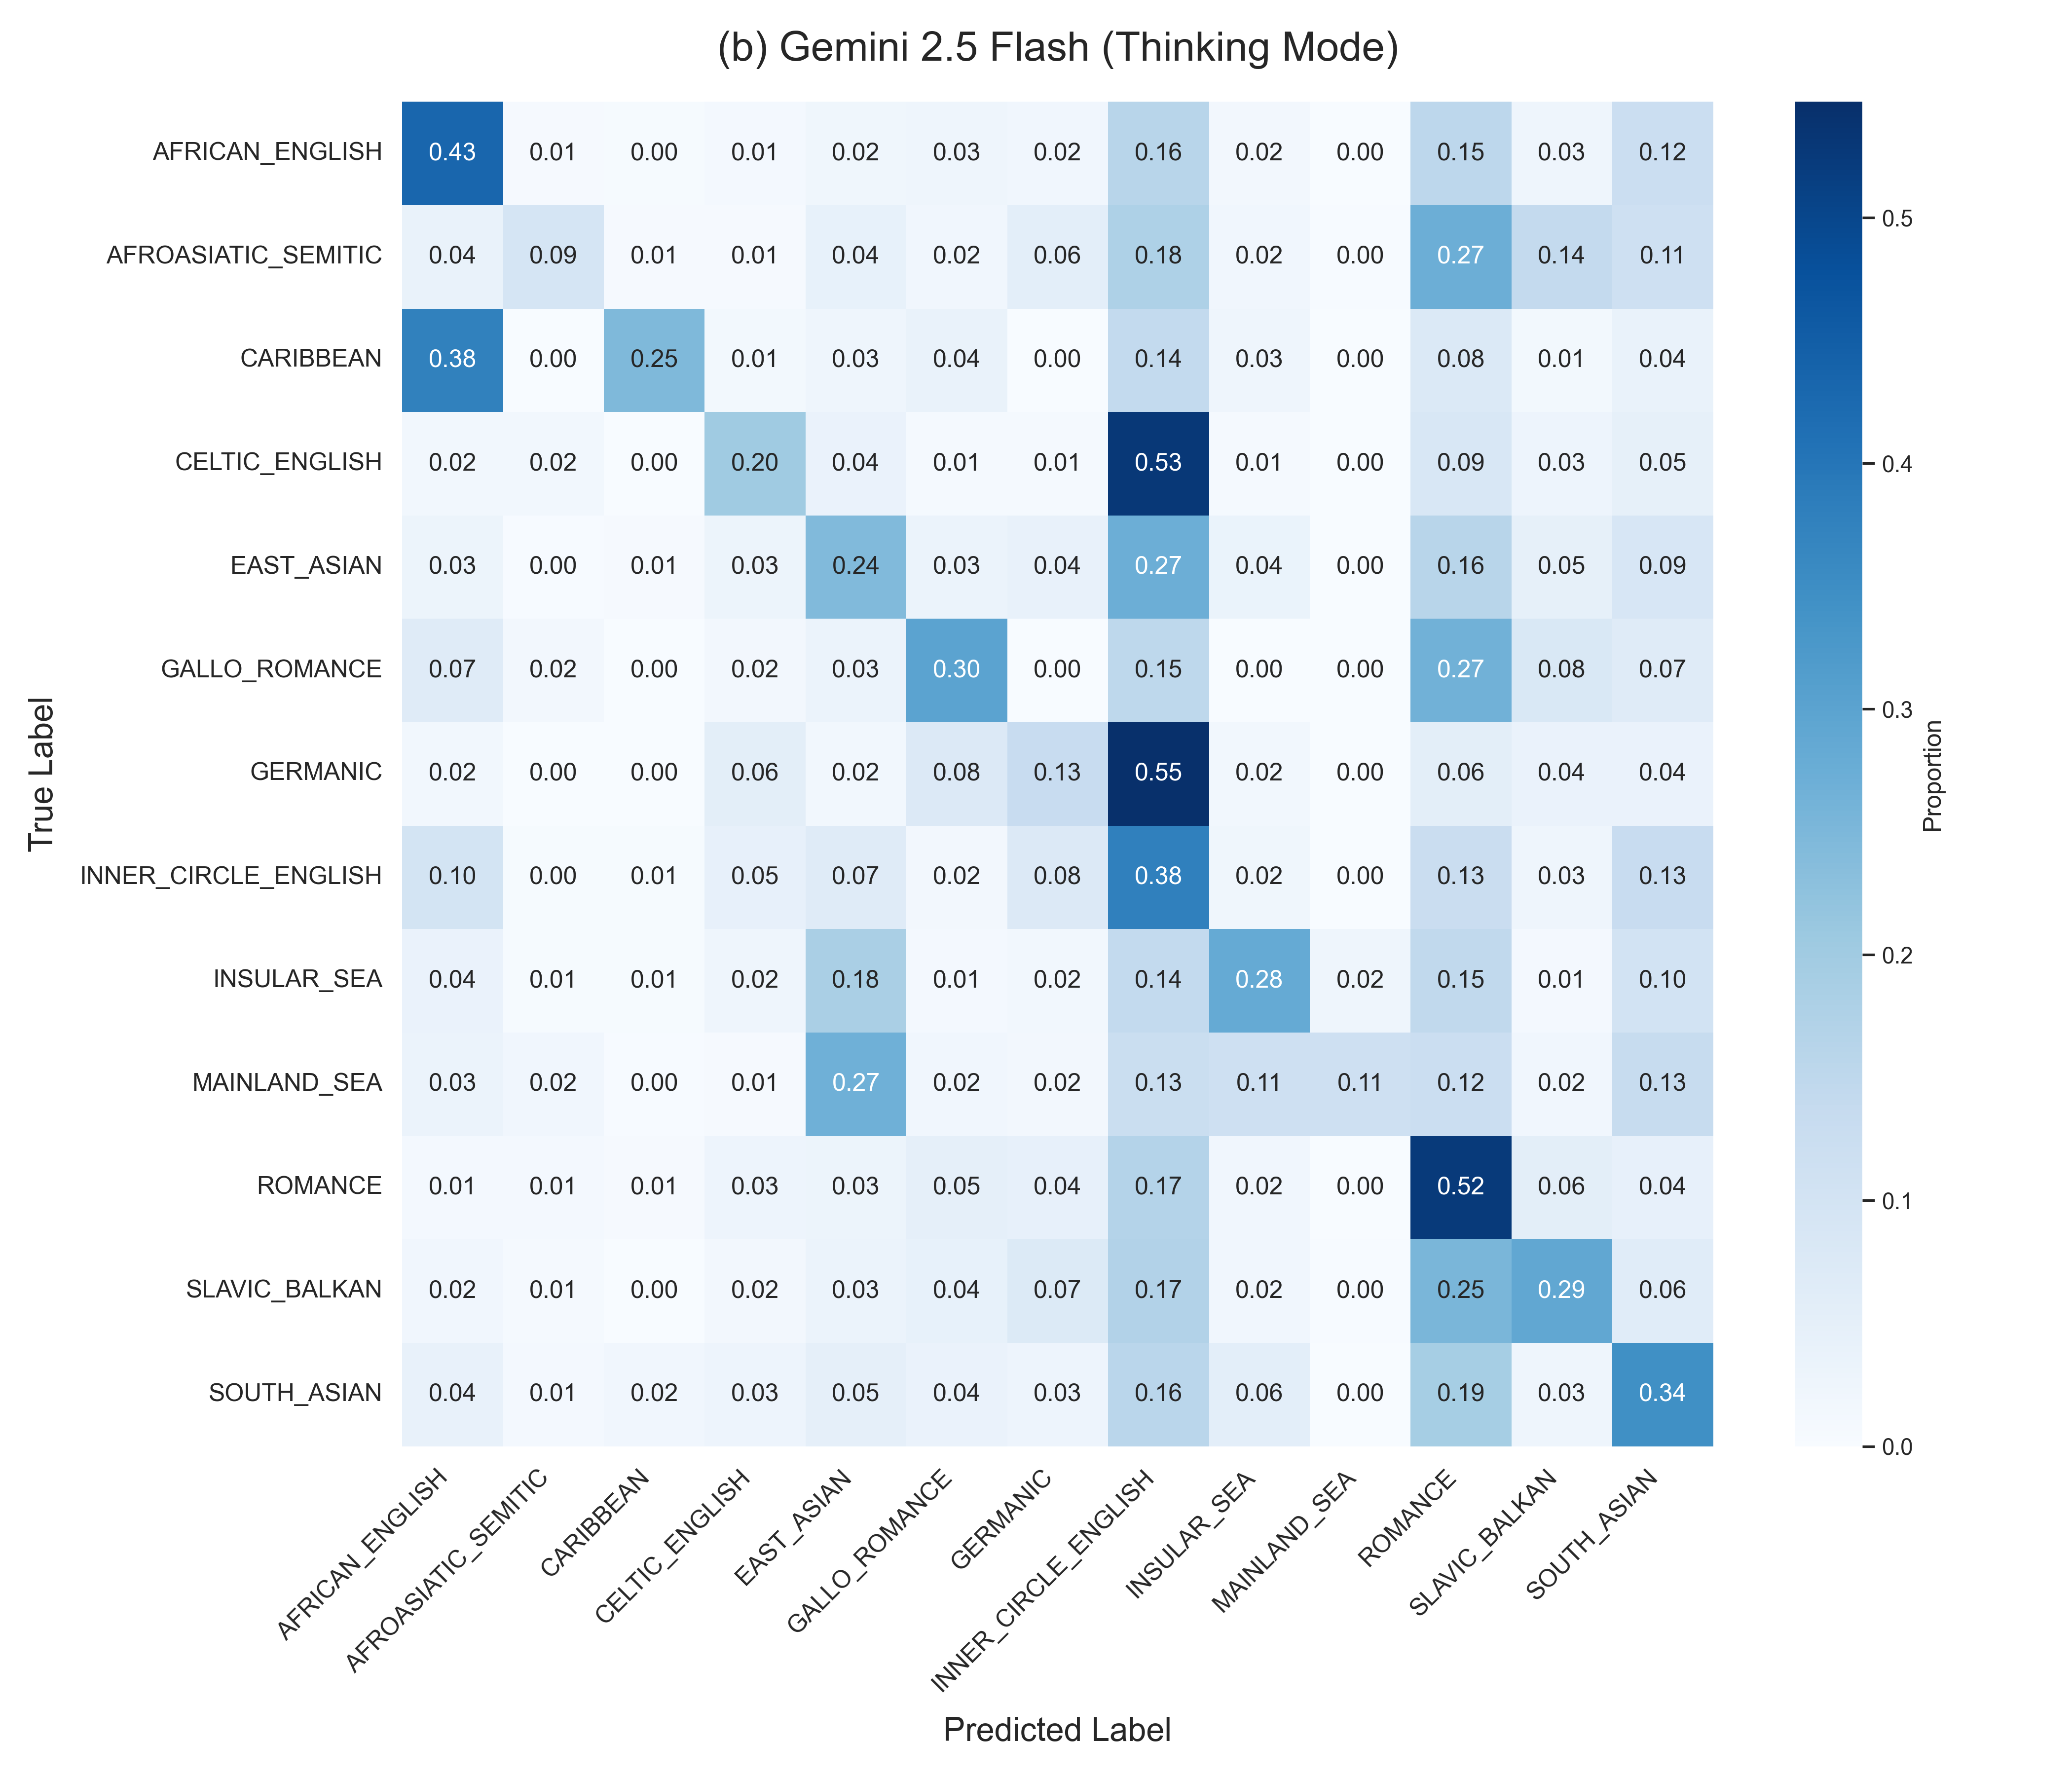
\includegraphics[width=\textwidth]{figures/cm_gemini_thinking.png}
    \caption{Thinking Mode (F1-score=24.9\%)}
  \end{subfigure}
  \caption{Normalized confusion matrices for Gemini 2.5 Flash on L1-eda (13 accent clusters). Rows denote true labels; columns denote predictions.}
  \label{fig:lalm-cm}
\end{figure}